\documentclass[../../main.tex]{subfiles}
\begin{document}
\begin{oframed}
  \subfile{problem}
\end{oframed}

{\bf [解答]}

\begin{figure}[htb]
  \centering
  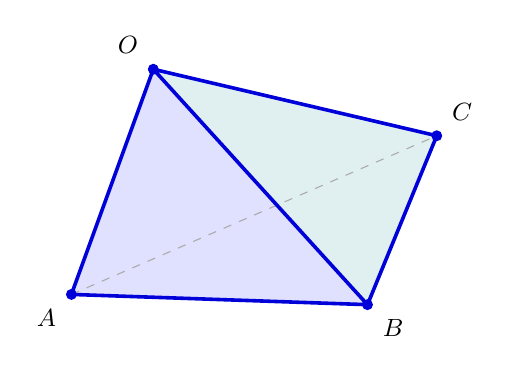
\begin{tikzpicture}[x=1.6cm, y=1.3cm, every node/.style={font=\small}]
    \coordinate (O) at (0.65,2.2);
    \coordinate (A) at (0,0);
    \coordinate (B) at (2.35,-0.1);
    \coordinate (C) at (2.9,1.55);
    \fill[blue!12] (O) -- (A) -- (B) -- cycle;
    \fill[teal!12] (O) -- (B) -- (C) -- cycle;
    \draw[dashed, gray!65] (A) -- (C);
    \draw[line width=1.3pt, blue!85!black] (O) -- (A) -- (B) -- (C) -- cycle (O) -- (B);
    \node[circle, fill=blue!85!black, inner sep=1.4pt] at (O) {}; \node[circle, fill=blue!85!black, inner sep=1.4pt] at (A) {}; \node[circle, fill=blue!85!black, inner sep=1.4pt] at (B) {}; \node[circle, fill=blue!85!black, inner sep=1.4pt] at (C) {};
    \node[above left=2pt] at (O) {$O$};
    \node[below left=2pt] at (A) {$A$};
    \node[below right=2pt] at (B) {$B$};
    \node[above right=2pt] at (C) {$C$};
  \end{tikzpicture}
  \caption{四面体$OABC$}
\end{figure}

点$X$に対し，$\overrightarrow{OX}=\vec x$と定める．条件(i)から
\begin{align}
  \begin{cases}
    \vec a\cdot(\vec c-\vec b)=0\\
    \vec b\cdot(\vec c-\vec a)=0\\
    \vec c\cdot(\vec b-\vec a)=0
  \end{cases} \label{eq:1}
\end{align}
である．

次に条件(ii)から，$\triangle OAB, OBC,OCA,ABC$の面積を$T$として，
\begin{align}
  T
  &=\dfrac{1}{2}\sqrt{|\vec a|^2|\vec b|^2-(\vec a\cdot\vec b)^2}\\
  &=\dfrac{1}{2}\sqrt{|\vec b|^2|\vec c|^2-(\vec b\cdot\vec c)^2}\\
  &=\dfrac{1}{2}\sqrt{|\vec c|^2|\vec a|^2-(\vec c\cdot\vec a)^2}\\
  &=\dfrac{1}{2}\sqrt{|\vec b-\vec a|^2|\vec c-\vec a|^2-\{(\vec b-\vec a)\cdot(\vec c-\vec a)\}^2} \label{eq:2}
\end{align}
である．

\cref{eq:1}より
\begin{align}
  \vec a\cdot\vec b=\vec b\cdot\vec c=\vec c\cdot\vec a \equiv q \label{eq:3}
\end{align}
とおけて，\cref{eq:2}に代入すると
\begin{align}
  |\vec a|^2|\vec b|^2=|\vec b|^2|\vec c|^2=|\vec c|^2|\vec a|^2
\end{align}
が従う．$|\vec a|,|\vec b|,|\vec c|>0$から，
\begin{align}
  |\vec a|=|\vec b|=|\vec c| \equiv p \label{eq:4}
\end{align}
となる．

\cref{eq:2}で$\triangle ABC, OAB$の面積を$p,q$で表すと
\begin{align}
  T
  &=\dfrac{1}{2}\sqrt{4(p^2-q)^2-(p^2-q)^2}\\
  &=\dfrac{1}{2}\sqrt{p^4-q^2}
\end{align}
だから，平方根の中身が等しく，
\begin{align}
  & 4(p^2-q)^2-(p^2-q)^2=p^4-q^2\\
  & 3(p^2-q)^2=p^4-q^2\\
  & 2p^4-6p^2q+4q^2=0\\
  & (p^2-2q)(2p^2-2q)=0 \\
  \therefore\
  & q=\dfrac{1}{2}p^2,\ p^2 \label{eq:5}
\end{align}
である．ここで$q = \vec{a}\cdot\vec{b}=|\vec{a}||\vec{b}|\cos\angle AOB = p^2 \cos\angle AOB$であり，$0 < \angle AOB < \pi$より$|q|<p^2$だから
\begin{align}
  q=\dfrac{1}{2}p^2
\end{align}
が正しい．

この時
\begin{align}
  |\vec a-\vec b|=|\vec b-\vec c|=|\vec c-\vec a|=\sqrt{2p^2-p^2}=p
\end{align}
となり，\cref{eq:4}と合わせて四面体$OABC$は各辺の長さが等しく，正四面体である．\qed

{\bf [別解]}

\cref{eq:4}以下考えると，ベクトルの始点を$O$から$A$，$B$，$C$にとり直すことにより，
\begin{align}
  |\overrightarrow{AB}|=|\overrightarrow{BC}|=|\overrightarrow{CA}|=|\overrightarrow{OA}|
\end{align}
を得るから，\cref{eq:4}と合わせて四面体$OABC$は各辺の長さが等しく，正四面体である．\qed

\newpage

\end{document}
